%% For double-blind review submission, w/o CCS and ACM Reference (max submission space)
\documentclass[sigplan,10pt,review,anonymous]{acmart}
\settopmatter{printfolios=true,printccs=false,printacmref=false}
%% For double-blind review submission, w/ CCS and ACM Reference
%\documentclass[sigplan,review,anonymous]{acmart}\settopmatter{printfolios=true}
%% For single-blind review submission, w/o CCS and ACM Reference (max submission space)
%\documentclass[sigplan,review]{acmart}\settopmatter{printfolios=true,printccs=false,printacmref=false}
%% For single-blind review submission, w/ CCS and ACM Reference
%\documentclass[sigplan,review]{acmart}\settopmatter{printfolios=true}
%% For final camera-ready submission, w/ required CCS and ACM Reference
%\documentclass[sigplan]{acmart}\settopmatter{}

\usepackage{enumitem}
\usepackage{booktabs}
\usepackage{amssymb}
\usepackage{soul}
\usepackage{xspace}
\usepackage{color}
\usepackage{xcolor}
\usepackage{upquote}
\usepackage{listings}
\usepackage{amsmath}

\captionsetup[figure]{font=footnotesize,name={Fig.},labelfont={bf, footnotesize}}
\captionsetup[table]{font=footnotesize,name={Tab.},labelfont={bf, footnotesize}, skip=2pt, aboveskip=2pt}
\captionsetup{font=footnotesize,labelfont={bf, footnotesize}, belowskip=2pt}

\newcommand{\eg}{{\em e.g.}, }
\newcommand{\ie}{{\em i.e.}, }
\newcommand{\etc}{{\em etc.}\xspace}
\newcommand{\vs}{{\em vs.} }
\newcommand{\cmpn}{compartmentalization} 
\newcommand{\heading}[1]{\vspace{4pt}\noindent\textbf{#1}\enspace}
\newcommand{\ttt}[1]{\texttt{\small #1}}
\newcommand{\ttiny}[1]{\texttt{\scriptsize #1}}
\newcommand{\spol}[1]{\scriptsize{\sc#1}}
\newcommand{\pol}[1]{\texttt{\small {\color{purple}#1}}}
\newcommand{\rf}[1]{\ref{#1}}
\newcommand{\wka}{\ttt{a\textsubscript{1}}}
\newcommand{\wkq}{\ttt{q\textsubscript{1-4}}}

% For comments
\newcommand{\eat}[1]{}
\newcommand{\TODO}[1]{\hl{\textbf{TODO:} #1}\xspace}
\newcommand{\todo}[1]{\hl{#1}\xspace}
\newcommand{\nv}[1]{[{\color{cyan}#1 --- Nikos}]}
\newcommand{\review}[1]{{\color{red}#1}}

\definecolor{editorGray}{rgb}{0.95, 0.95, 0.95}
\definecolor{editorOcher}{rgb}{1, 0.5, 0} % #FF7F00 -> rgb(239, 169, 0)
\definecolor{editorGreen}{rgb}{0, 0.5, 0} % #007C00 -> rgb(0, 124, 0)

\definecolor{cdb}{rgb}{0.37, 0.62, 0.63} % cadet blue

\lstdefinelanguage{sh}{
  morekeywords={for, in, do, done, \|},
  keywordstyle=\color{purple}\ttfamily,
  % ndkeywords={curl, grep, wget, awk, xargs, find, nc, mdc, gunzip, cut, sort, head, join},
  ndkeywordstyle=\color{black}\ttfamily\bfseries,
  identifierstyle=\color{black},
  sensitive=false,
  comment=[l]{\#},
  commentstyle=\color{lightgray},
% morecomment=[s]{/\\*\\*, \\*/},
  stringstyle=\color{darkgray}\ttfamily,
  morestring=[b]',
  morestring=[b]",
% numbersep=1pt,
% numberstyle=\footnotesize\bf\color{gray},   % the style that is used for the line-numbers
  abovecaptionskip=0pt,
  aboveskip=0pt,
  belowcaptionskip=0pt,
  belowskip=0pt,
  frame=none                     % adds a frame around the code
% moredelim=[s][\color{gray}]{c:}{>},
% moredelim=[s][\color{orange}]{/*}{/}
}

\lstset{ %
  backgroundcolor=\color{white},   % choose the background color; you must add \usepackage{color} or \usepackage{xcolor}
  basicstyle=\small\ttfamily,  % the size of the fonts that are used for the code
  upquote=true,
  captionpos=b,                    % sets the caption-position to bottom
% frame=B,                    % adds a frame around the code
  numbers=left,                    % where to put the line-numbers; possible values are (none, left, right)
  numbersep=2pt,                   % how far the line-numbers are from the code
  numberstyle=\tiny\color{gray},   % the style that is used for the line-numbers
  rulecolor=\color{black},         % if not set, the frame-color may be changed on line-breaks within not-black text (e.g. comments (green here))
  framerule=0pt,
	xleftmargin=0pt,
	xrightmargin=0pt,
	breakindent=0pt,
  aboveskip=0pt,
  framesep=0pt,
  abovecaptionskip=0pt,
  aboveskip=0pt,
  belowcaptionskip=0pt,
  belowskip=0pt,
  frame=none,
  framexbottommargin=0pt,
  resetmargins=true
}



%% Conference information
%% Supplied to authors by publisher for camera-ready submission;
%% use defaults for review submission.
\acmConference[PL'18]{ACM SIGPLAN Conference on Programming Languages}{January 01--03, 2018}{New York, NY, USA}
\acmYear{2018}
\acmISBN{} % \acmISBN{978-x-xxxx-xxxx-x/YY/MM}
\acmDOI{} % \acmDOI{10.1145/nnnnnnn.nnnnnnn}
\startPage{1}

%% Copyright information
%% Supplied to authors (based on authors' rights management selection;
%% see authors.acm.org) by publisher for camera-ready submission;
%% use 'none' for review submission.
\setcopyright{none}
%\setcopyright{acmcopyright}
%\setcopyright{acmlicensed}
%\setcopyright{rightsretained}
%\copyrightyear{2018}           %% If different from \acmYear

%% Bibliography style
\bibliographystyle{ACM-Reference-Format}
%% Citation style
%\citestyle{acmauthoryear}  %% For author/year citations
%\citestyle{acmnumeric}     %% For numeric citations
%\setcitestyle{nosort}      %% With 'acmnumeric', to disable automatic
                            %% sorting of references within a single citation;
                            %% e.g., \cite{Smith99,Carpenter05,Baker12}
                            %% rendered as [14,5,2] rather than [2,5,14].
%\setcitesyle{nocompress}   %% With 'acmnumeric', to disable automatic
                            %% compression of sequential references within a
                            %% single citation;
                            %% e.g., \cite{Baker12,Baker14,Baker16}
                            %% rendered as [2,3,4] rather than [2-4].


%%%%%%%%%%%%%%%%%%%%%%%%%%%%%%%%%%%%%%%%%%%%%%%%%%%%%%%%%%%%%%%%%%%%%%
%% Note: Authors migrating a paper from traditional SIGPLAN
%% proceedings format to PACMPL format must update the
%% '\documentclass' and topmatter commands above; see
%% 'acmart-pacmpl-template.tex'.
%%%%%%%%%%%%%%%%%%%%%%%%%%%%%%%%%%%%%%%%%%%%%%%%%%%%%%%%%%%%%%%%%%%%%%


%% Some recommended packages.
\usepackage{booktabs}   %% For formal tables:
                        %% http://ctan.org/pkg/booktabs
\usepackage{subcaption} %% For complex figures with subfigures/subcaptions
                        %% http://ctan.org/pkg/subcaption


\begin{document}

%% Title information
\title{Distribution-oblivious Programming with Dish}         %% [Short Title] is optional;
% \titlenote{with title note}             %% \titlenote is optional;
%                                         %% can be repeated if necessary;
%                                         %% contents suppressed with 'anonymous'
% \subtitle{Subtitle}                     %% \subtitle is optional
% \subtitlenote{with subtitle note}       %% \subtitlenote is optional;
                                        %% can be repeated if necessary;
                                        %% contents suppressed with 'anonymous'


%% Author information
%% Contents and number of authors suppressed with 'anonymous'.
%% Each author should be introduced by \author, followed by
%% \authornote (optional), \orcid (optional), \affiliation, and
%% \email.
%% An author may have multiple affiliations and/or emails; repeat the
%% appropriate command.
%% Many elements are not rendered, but should be provided for metadata
%% extraction tools.

%% Author with single affiliation.
\author{First1 Last1}
\authornote{with author1 note}          %% \authornote is optional;
                                        %% can be repeated if necessary
\orcid{nnnn-nnnn-nnnn-nnnn}             %% \orcid is optional
\affiliation{
  \position{Position1}
  \department{Department1}              %% \department is recommended
  \institution{Institution1}            %% \institution is required
  \streetaddress{Street1 Address1}
  \city{City1}
  \state{State1}
  \postcode{Post-Code1}
  \country{Country1}                    %% \country is recommended
}
\email{first1.last1@inst1.edu}          %% \email is recommended

%% Author with two affiliations and emails.
\author{First2 Last2}
\authornote{with author2 note}          %% \authornote is optional;
                                        %% can be repeated if necessary
\orcid{nnnn-nnnn-nnnn-nnnn}             %% \orcid is optional
\affiliation{
  \position{Position2a}
  \department{Department2a}             %% \department is recommended
  \institution{Institution2a}           %% \institution is required
  \streetaddress{Street2a Address2a}
  \city{City2a}
  \state{State2a}
  \postcode{Post-Code2a}
  \country{Country2a}                   %% \country is recommended
}
\email{first2.last2@inst2a.com}         %% \email is recommended
\affiliation{
  \position{Position2b}
  \department{Department2b}             %% \department is recommended
  \institution{Institution2b}           %% \institution is required
  \streetaddress{Street3b Address2b}
  \city{City2b}
  \state{State2b}
  \postcode{Post-Code2b}
  \country{Country2b}                   %% \country is recommended
}
\email{first2.last2@inst2b.org}         %% \email is recommended

\newcommand{\cf}[1]{(\emph{Cf}.\S\ref{#1})}
\newcommand{\sx}[1]{(\S\ref{#1})}
\newcommand{\sys}{{\scshape Dish}\xspace}
\newcommand{\unix}{{\scshape Unix}\xspace}

\setlist{noitemsep,leftmargin=10pt,topsep=2pt,parsep=2pt,partopsep=2pt}

%% Abstract
%% Note: \begin{abstract}...\end{abstract} environment must come
%% before \maketitle command
\begin{abstract}
  \nv{placeholder}
  Distributed systems offer notable benefits over centralized ones.
  Reaping these benefits, however, requires programming in a way that makes distribution explicit---\eg via new programming languages, distributed framework interfaces, or distribution annotations.
% 
%   \emph{Distribution-oblivious programming} is a new approach for..?
  This paper presents \sys, a shell variant that automatically and correctly scales out distribution-oblivious shell pipelines. %  with regards to the sequential program.
  % leveraging the insight that such programs already express stream computations, with their stages falling under a few, known distributability classes.
  \sys's insight is that shell pipelines already express stream computations that can automatically distributed.
  To achieve this, \sys
% a series of techniques for automatically 
decomposes primitives into distributability classes,
identifies high-distributability stages,
applies rewriting rules for largest possible subprograms,
and orchestrates the distributed program.
Its runtime component provides orchestration and planning support during the execution of the program.
% 
% Key challenges include 
% surprisingly expressive, 
% maximally distributable subprograms
% 
Experiments for complex pipelines show substantial speedups and the ability to operate on large input datasets, all without any developer input.
\end{abstract}


%% 2012 ACM Computing Classification System (CSS) concepts
%% Generate at 'http://dl.acm.org/ccs/ccs.cfm'.
\begin{CCSXML}
<ccs2012>
<concept>
<concept_id>10011007.10011006.10011008</concept_id>
<concept_desc>Software and its engineering~General programming languages</concept_desc>
<concept_significance>500</concept_significance>
</concept>
<concept>
<concept_id>10003456.10003457.10003521.10003525</concept_id>
<concept_desc>Social and professional topics~History of programming languages</concept_desc>
<concept_significance>300</concept_significance>
</concept>
</ccs2012>
\end{CCSXML}

\ccsdesc[500]{Software and its engineering~General programming languages}
\ccsdesc[300]{Social and professional topics~History of programming languages}
%% End of generated code


%% Keywords
%% comma separated list
% \keywords{keyword1, keyword2, keyword3}  %% \keywords are mandatory in final camera-ready submission


%% \maketitle
%% Note: \maketitle command must come after title commands, author
%% commands, abstract environment, Computing Classification System
%% environment and commands, and keywords command.
\maketitle


\section{Introduction}

% 1. Shell scripting; pipelines, in particular, are a common abstraction for expressing filters
% They are an easy way to , because they combine a set of assumptions that work well with Unix
% They work great on a single machine, but are difficult to scale out
% Could we fully automate distribution? 
% The key insight is that pipelines already express a domain-specific
% computation that is easily amenable to distribution.
% 

Distributed systems offer significant benefits over their centralized counterparts---for example, they can speed up expensive computations or process data that would not fit into any single machine.
% offer notable benefits over their centralized counterparts:
%   using partitioning and replication, they can process and store data with increased throughput and fault-tolerance.
% Yet, only a minority of developers, employed by the select few companies that deal with massive datasets, have the luxury of engineering software systems with distribution baked in from the start.
% The remaining majority starts by developing and deploying software in a centralized manner---that is, \emph{until} there is a significant change of requirements, such as a load increase.
Despite these benefits, their development remains different from and significantly more difficult than their centralized counterparts.
Whereas anyone can quickly stitch together a Bash script to compute on a single computer, 
  % domain-experts routinely glue scripts together to process and share data. % without the help of a computing expert.
   scaling out to multiple ones requires expert labor around ``point'' solutions with expensive setups, restricted programming interfaces, and exorbitant composition costs~\cite{taurus:14, dios:13, andromeda:15, pywren:17, futuredata:18, nefele:18}.

To understand this sharp contrast, consider calculating term frequencies over a set of input files:

% \begin{lstlisting}[language=sh,float=h,numbers=none]
% cat doc.ms |                   # print input file
% groff -t -e -mandoc -Tascii |  # remove formatting
% col -bx |                      # remove backspaces 
% tr A-Z a-z |                   # convert to lower case
% tr -d '[:punct:]' |            # remove punctuation
% sort |                         # put words in alphabetical order
% unique |                       # remove duplicate words
% comm -13 /usr/share/dict -     # report words not in dictionary 
% \end{lstlisting}

\begin{lstlisting}[language=sh, float=h, numbers=none, escapeinside={($}{$)}]
cat * | tr -cs A-Za-z\n | tr A-Z a-z |    ($$[p_1]$$)
  sort | uniq -c | sort -rn | head 5 > out
\end{lstlisting}

\noindent
Program $p_1$ creates a character stream, breaks it into words, transliterates to lower-case, sorts to group duplicates, summarizes them with a counter, sorts them in descending order, picks the top five results and writes them to a file \ttt{out}.
Combining several features, \unix makes small tasks easy to express;
  for a user with \emph{one} computer and small input, this pipeline takes a few seconds to compose and execute~\cite{bentley1986literate}.
% composition allows the composition of general primitives

% Key insight 
% % The garden-hose philosophy is similar to Haskell 
% This pipeline takes an input file (line 1), removes 
% * do not need to use specialized frameworks for composition---instead, as long as they conform to the shell, individual primitives can be written in any programming language.
% * do not need to rewrite ---

\begin{figure}[t]
\centering
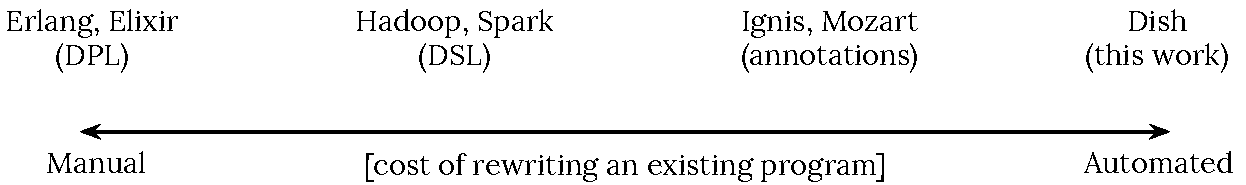
\includegraphics[width=0.49\textwidth]{./figs/dish_spectrum.pdf}
\caption{
  \textbf{Cost of Manual Effort.}
	\sys sits at the automation end of the spectrum, automatically distributing shell pipelines while maintaining their correctness. A more complete picture is presented in the related-work section~\sx{rt}.
}
\label{fig:spectrum}
\end{figure}


%      dish      ignis, mozart    hadoop, spark, ...      erlang, elixir
%       \/           \   /             \     /                \   /
% auto <-------------------------------------------------------------> manual
%                      [rewrite (not write) cost]

For a user with many computers and larger inputs, however, developing $p_1$'s distributed equivalent requires a significant effort.
% The scope of such rewrites, and therefore the cost of manual effort, can vary considerably.
For simple pipelines that capture in restricted models of computation, this effort amounts to expressing the computation using the primitives provided by a big-data framework~\cite{mapreduce:08, ciel:11, spark:12, naiad:13} or domain-specific language~\cite{alvaro2011consistency, distal:13, meiklejohn2015lasp}---an unjustifiable cost for one-off pipelines that take a few minutes to compose (but are applied to large datasets).
More complex pipelines, such as the ones presented in later sections, require full-fledged distributed programming language~\cite{erlang:96, lopes1997d, acute:05, mace:07, cloudhaskell:11, ScalaLoci:18}. %  or a distributed operating system---\eg Plan9's \ttt{rc} shell.
In these cases, manual rewriting is expensive and can introduce new bugs, cascading changes, or divergence from legacy functionality.
Could the generation and execution of $p_1$'s distributed version be fully and correctly automated?

% Some (parts of) pipelines require only moderate effort, as they are 
% For some pipelines, this effort is merely moderate, as 
%  can be expressed in domain-specific frameworks---for example, Hadoop and Spark provide a few purely functional primitives that 
%   ---still requiring rewriting the program in a different (\eg Scala for Spark).
% 
% This effort is moderate if the program expressed by these pipelines fits into a domain-specific framework.
% At times, such pipelines
% As long as the program fits into the model this is only moderately difficult;
% 
% For many legacy pipelines  
%  has to choose between three options, all of which require significant manual effort.
% The most invasive is to rewrite the entire program in a distributed programming language
% The most popular is to leverage 
% 
% Use a distributed programming language, even higher rewrites
% Or use some form of annotations 
% 
%  this requires rewriting portions of the program in a new language and use operations
% 
% 
% In the simplest case, annotations
% 
% Often, they only focus on a few parts of the system---for example, upgrading to a distributed storage layer.
% More rarely, companies rewrite entire systems (\eg Twitter's Ruby-to-Scala rewrite~\cite{twitter}), a process that is notoriously difficult under schedule constraints and competitive pressures~\cite{rewrite1, rewrite2}.
%  especially since software today makes extensive use of third-party modules~\cite{breakapp:plos:2017}.
% 

% If developers have already expressed their computation as a Unix pipeline, they should not have to manually rewrite the program in other environment---\eg Hadoop, Spark---to exploit distribution.


The key insight behind \sys is that the language of the Unix shell already encodes stream processing, providing most of the information required for distributing a computation.
\sys builds on this insight with a careful study of the scalability properties of shell primitives and its commands, paired with a novel rewriting scheme that identifies maximal pipeline sub-expressions that are candidates for scale-out.
We term the result \emph{distribution-oblivious programming}---a series of techniques that fully automates program distribution while provably maintaining correct (non-distributed) semantics.

Key benefits include the ability to scale legacy computations onto
\sys converts legacy shell pipelines into their distributed equivalents fully automatically, offering $100\times$ improvements in performance without a single line of additional code or annotation.
Most importantly, \sys provides an architectural lesson:
  the current design shows that large-scale efforts in the distributed- and operating-system literature to provide a \unix-like distributed equivalent could have been simplified by a thin (but sophisticated) rewriting shim like the one \sys provides.

% % Make Unix benefits explicit?
% Indeed, the primary reason behind $p_1$'s succinctness is that the pipeline is a domain-specific language for describing operations over streams.
% Key elements of \unix are the ability to compose programs written in different languages, the abstraction of a file system as a set of resident streams, a small but extensible library of commands, and the ability to resolve names within a global context.
% Under the hood, the \unix kernel buffers results, synchronizes processing stages, and generally orchestrates the computation.

% Primitives 
% \sys enables \emph{distribution-oblivious programming}: 
%   multi-order of magnitude speedups with correctness guarantees and without any developer effort.
% 
% The a series of transformations that 
% Second, we are using describing composition . For this, we are restricting the study to a subset of the POSIX shell--
% 
% Local operations and identifiers have to be carefully translated to distributed ones, a translation that depends on the types of the operations and associated identifiers.
% 
% The semantics is enough to capture powerful features such as stream branching and feedback constructs found in practice and in the system's evaluation.

The paper is structured as follows.
We first start with a background section outlining pipeline concepts~\sx{bg}.
Sections \ref{classes}--\ref{recipes} highlight our key contributions:\footnote{
  This is not precise, we'll need to wait until it matures a bit.
}
\begin{itemize}

  \item
  \S\ref{classes} overviews \sys and introduces several scalability and distributability classes.

  \item
  \S\ref{rewrite} presents a set of rewriting transformations for identifying maximal pipeline sub-expressions, candidates for scale-out.

  \item
  \S\ref{other} details other concerns, such as distributed state management and extensibility.
\end{itemize}

\noindent
\sys's evaluation~\sx{eval} uses a combination of one-liner micro-benchmarks that highlight certain features and three multi-line macro-benchmarks---a web crawling and indexing engine, a production genomics pipeline, and a large-scale weather analysis.
We close with a discussion of related prior work~\sx{related} and possible future directions~\sx{discussion}.

\begin{figure*}[t]
\centering
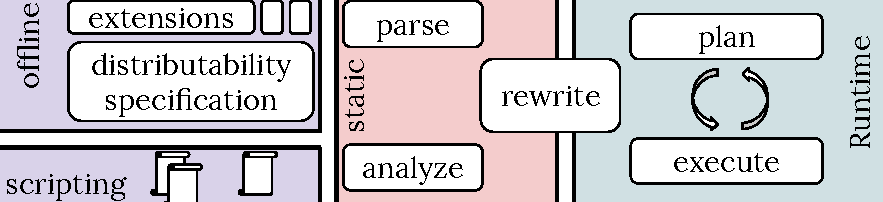
\includegraphics[width=0.49\textwidth]{./figs/dish_overview.pdf}
\caption{
  \textbf{Applying \sys to $p_1$.}
}
\label{fig:example}
\end{figure*}


\section{Background}
\label{bg}

This section breaks down $p_1$ to presents important background on and challenges
of shell scripting.

\subsection{Unix Pipelines, Informally}
\label{bg:pipelines}

Pipelines are a mechanism for program composition.
Individual programs, specified as commands, conform to a common but general interface. 
For now, this interface allows a combination of the following:
  accepting input from the standard input stream (stdin),
  generating output to the standard output stream (stdout), and
  generating errors or diagnostics to the standard error stream (stderr)
Standard streams are streams of characters with a few special characters---for example, EOF is a special end-of-file character signaling the end of the input stream.
% For Unix commands, the newline character is special; as such, Unix streams can be seen as lazy lists of strings---lines of text separated by the newline character.

Leveraging this interface, pipelines chain together commands by their standard streams, such that the output stream of one command (stdout) is passed directly as input (stdin) to the next one.
Pipeline chaining goes hand-in-hand with the Unix toolbox philosophy: 
  programs do one thing well, they work together, and they manipulate text streams as their universal interface.
The next few paragraphs describe the details.


\heading{Basics}
The standard shell syntax for pipelines a list of commands separated by vertical bars (``pipes'', in Unix terminology).

that are not interpreted by the shell, but are local to each command.

Additional details augment this simple interface.
Commands can be specified with options arguments

\begin{figure}[t]
\centering
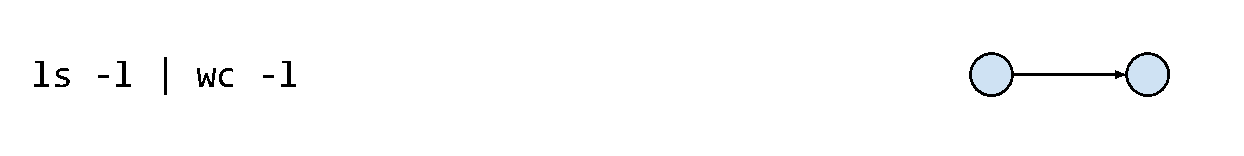
\includegraphics[width=0.45\textwidth]{./figs/dish_ex1.pdf}
\label{fig:example}
\end{figure}


\begin{lstlisting}[language=sh, float=h, numbers=none, escapeinside={($}{$)}]
 ls -l | wc -l                           (($$p_2$$))
\end{lstlisting}

\heading{Generation}
A central concept in pipelines---and Unix, in general---is the file system, which allows interfacing with persistent data.
There are many commands that take as input a file identifier 
Reading a file or a set of files generates a stream; 
  similarly, streams can be trivially redirected to the file system---by appending with the file identifier.

Expansion---the key is that expansion and evaluation are handled by the shell at an earlier stage 
The most powerful---and interesting, for \ttt{dish}---type of expansion is subshell expansion, that allows replacing entire input streams 


\begin{lstlisting}[language=sh, float=h, numbers=none, escapeinside={($}{$)}]
 cat * | wc -l > out.txt                 (($$p_3$$))
\end{lstlisting}

\heading{Identifiers}

The file-system is a common abstraction layer used for many other operations than just serving files (this will be become clearer when talking about file-system commands in \S\ref{bg:cmd}).
as such, different identifiers many not resolve to actual files, but rather in-memory or OS-internal structures.

At a high level, POSIX defines several file types:
(-) regular files, storing lines of text or binary data,
(d) directories, grouping together multiple other files,
(l) symbolic links, pointing to other files,
(p) named pipes or FIFOs, communication primitives that can be named and manipulated like files,
(s) domain sockets or DSes, full-duplex communication primitives that support passing file descriptors, and
(b or c) special files, interfaces to device drivers or low-level abstractions, presented as ordinary files.

Most of these identifiers are manipulated by file-system commands---\eg \ttt{mkdir} for directories and \ttt{mkfifo} for FIFOs.
FIFOs and DSes look like files but are streams.

Special files are particularly interesting because they are resolved to OS structures.
One set is pseudo-devices---device files that simply;
For example /dev/urandom returns a stream of random characters and /dev/null accepts and discards all input written to it.
Another set is proc filesystem (procfs), a special filesystem in Unix-like operating systems that presents information about processes and other system information.
For example, /proc/PID/cmdline contains command that originally started the process and /proc/PID/cwd contains a symlink to the current working directory of the process.

sysfs is a pseudo file system provided by the Linux kernel that exports information about various kernel subsystems, hardware devices, and 

/modules, one of the most important files in /proc, containing a list of the kernel modules currently loaded . It gives some indication (not always entirely correct) of dependencies.
/cpuinfo

symbolic links, FIFO specials, 
device files
block special, character special, 
and domain sockets.

There are 3 standard streams (stdin, stdout, stderr) created automatically for most Unix programs.
These correspond to \ttt{/dev/fd/0}.
% These streams are created by the C library (glibc) at the start of program execution,
and new streams can be created to connect to files, sockets, pipes,

Unix already specifies a few classes of files:

Here are a few special files:
  \ttt{proc} called 

Technically, anonymous pipes show up as file identifiers in a hidden filesystem.
Similarly, open files and other ephemeral identifiers 


\begin{lstlisting}[language=sh, float=h, numbers=none, escapeinside={($}{$)}]
 cat /proc/ >                            (($$p_4$$))
\end{lstlisting}

\heading{Stream Manipulation}
A small but powerful set of primitives are concerned with stream manipulation.
First, as described above, several commands can be redirected
Second, 

\ttt{xargs}
\ttt{tee}

In combination, these constructs are powerful enough to introduce circular streams. % or stream cycles?

Explicit Redirection
Implicit splitting and merging 
This can be done through the file-system operators 

\begin{lstlisting}[language=sh, float=h, numbers=none, escapeinside={($}{$)}]
 cat /proc/ >                            (($$p_5$$))
\end{lstlisting}

\heading{Composition}
anonymous pipes

Composition

The shell provides several ways of grouping commands and manipulating their
overall input and output channels 

{ echo 1; echo 2; } > out.txt

\subsection{Comnands}
\label{bg:cmd}

% Sets vs. Classes

Distributability classes, based on how 

\heading{Preliminaries}

\heading{POSIX, GNU Core-utils, and beyond}

\heading{Stateless}

\heading{Pure}

\heading{File-system}

\heading{Side-effectful}

\heading{Irreversably Side-effectful}

\subsection{The Shell Language}
\label{bg:shell}

\heading{Implicits}
Expansion
Implicits
Context

\heading{Language Constructs}

Even without these, the Unix pipeline language is powerful enough to capture complex pipelines.

We can encode powerful

\section{Dish Overview}

\section{Related Work}

\begin{acks}
  % Dumping people so that we don't forget
  % 
  This material is based upon work supported by the
  \grantsponsor{GS100000001}{National Science
    Foundation}{http://dx.doi.org/10.13039/100000001} under Grant
  No.~\grantnum{GS100000001}{nnnnnnn} and Grant
  No.~\grantnum{GS100000001}{mmmmmmm}.  Any opinions, findings, and
  conclusions or recommendations expressed in this material are those
  of the author and do not necessarily reflect the views of the
  National Science Foundation.
\end{acks}


%% Bibliography
\bibliography{./bib}


%% Appendix
\appendix
\section{Scripts used in the evaluation}

This appendix contains the source code of the scripts used in the evaluation of
the \sys. They are part of the codebase (released as open source with the camera
ready), and are provided here only to aid the reviewers.


\end{document}
